
Aufgabe der Replikation von CouchDB ist die Synchronisation 2+n Datenbanken. Lösungen: Zuverlässige \b{Synchronisation} von Datenbanken auf verschiedenen Geräten. \b{Verteilung} der Daten über ein Cluster von DB-Instanzen die jeweils einen Teil des requests beantworten (Lastverteilung) und \b{Spiegelung} der Daten über geografisch weit verteilte Standorte.\\
Durch die inkrementelle (schrittweise) Arbeitsweise kann CouchDB genau dort weitermachen wo es unterbrochen wurde wenn während der Replikation ein Fehler auftritt, beispielsweise durch eine ausfallende Netzwerkverbindung
\it{Es werden auch nur die Daten übertragen, die notwendig sind, um die Datenbanken zu synchronisieren.}\\
Das Besondere an CouchDB ist, dass es darauf ausgerichtet ist, Fehler/Konflikte vernünftig zu behandeln statt anznehmen es träten keine auf (vgl. \cite{couchDB} S. 7f). Wie \hyperref[chap:conflict]{oben} beschrieben, gibt es in Verteilten Systemen einige Fehler die auftreten können.\\\\
\it{Das CouchDB Replikationsmodell erlaubt eine nahtlose, peer-to-peer (direkte) Datensynchronisation zwischen beliebig vielen Geräten. Das CouchDB Replikationsprotokoll ist in CouchDB selbst implementiert, das die Serverkomponente abdeckt. Dann gibt es das PouchDB-Projekt, das dasselbe Protokoll in JavaScript implementiert, das auf Browser- und Node.js-Anwendungen abzielt. das deckt Ihre Kunden und dev-Server ab. Schließlich gibt es Couchbase Mobile und Cloudant Sync, die auf iOS und Android laufen und das CouchDB Synchronisationsprotokoll in Objective-C bzw. Java implementieren.}\\
content addressable versions: Idee: Nimm den Objektinhalt (content) und jag ihn durch eine \gls{Hashfunktion}\\
%
Diese Art von Konflikten sollten von Menschen gelöst werden. Nur so kann sichergestellt werden, dass die korrekte Änderung gespeichert wird und keine Daten verloren gehen.
%
% \subsub{schlussendliche Konsistenz}
\subsub{Eventual Consistency}
\todo{Das muss noch woanders hin. oder raus}\\
Das \gls{CAP} Theorem, veranschaulicht in \autoref{fig:cap}, besagt, dass jedes System mit dem Daten über das Netzwerk gesendet werden, nur zwei von den drei möglichen Eigenschaften, Konsistenz, Verfügbarkeit und Partitionstoleranz, garantieren kann.
Konsitzenz der gespeicherten Daten bedeutet, es muss sichergestellt werden dass nach Abschluss der Transaktion auch alle Replikate des manipulierten Datensatzes aktualisiert werden. Der Datensatz ist in jeder Datenbank identisch.
%
\begin{figure}[H]
  \centering
  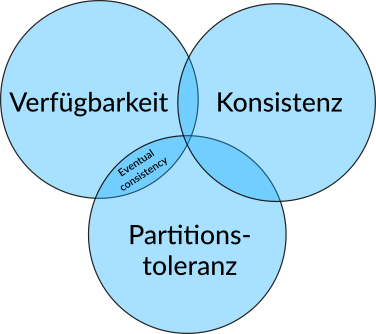
\includegraphics[width=0.6\textwidth]{cap}
  \grayRule
  \caption{Das CAP Theorem}
  \label{fig:cap}
\end{figure}
%
Das System ist besitzt eine hohe Verfügbarkeit wenn alle Anfragen an das System stets beantwortet werden. Die Verfügbarkeit ist gering, wenn die Antwortzeiten des Systems lang sind.
Partitionstoleranz ist gleichzusetzen mit Ausfalltoleranz. Die Datenbank kann auf mehreren Servern verteilt sein. Trotzdem ein Server oder eine Partition ausfällt, kann das System weiterhin funktionieren.\\
Eventual Consistency kommt häufig bei verteilten Datenbanken zur Anwendung und stellt die Konsitenz der Daten nach einem gewissen Zeitfenster sicher (vgl. ~\cite{couchDB} S. 11 ff.). 
% Wenn Verfügbarkeit Priorität hat, können wir Clients die Daten zunächst auf einen Knoten schreiben lassen, ohne darauf zu warten, dass die anderen Knoten synchronisiert werden.
% Wenn die Datenbank weiß, wie sie mit dieser Situation umzugehen hat, sind die Daten irgendwann „letztendlich konsistent“ — allerdings unter Aufgabe der Hochverfügbarkeit der Daten.
% Für viele Anwendungen ist das ein erstaunlich guter Kompromiss.
\subsub{Lokale Konsistenz}
\subsub{Verteilte Konsistenz}

\subsub{Replikation?}
\subsub{Konfliktmanagement}
